\documentclass[border=4pt]{standalone}
\usepackage{tikz}
\usetikzlibrary{arrows,positioning}
\begin{document}
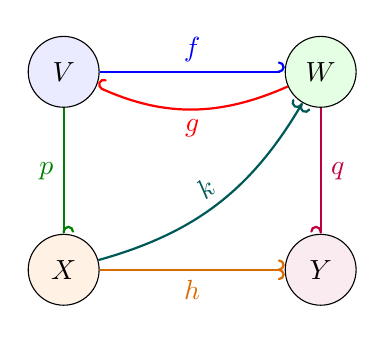
\begin{tikzpicture}[
  node distance=1.6cm and 2.35cm,
  obj/.style={draw,circle,minimum size=9mm,inner sep=1pt}
]
  \node[obj,fill=blue!8] (V) {$V$};
  \node[obj,fill=green!10,right=of V] (W) {$W$};
  \node[obj,fill=orange!10,below=of V] (X) {$X$};
  \node[obj,fill=purple!8,right=of X] (Y) {$Y$};

  \draw[blue,line width=.8pt,-{left hook}] (V) -- node[above] {$f$} (W);
  \draw[red,line width=.8pt,-{right hook}] (W) to[bend left=24] node[below] {$g$} (V);
  \draw[green!50!black,line width=.8pt,-{left hook reversed}] (V) -- node[left] {$p$} (X);
  \draw[purple,line width=.8pt,-{right hook reversed}] (W) -- node[right] {$q$} (Y);
  \draw[orange!85!black,line width=.8pt,-{hooks}] (X) -- node[below] {$h$} (Y);
  \draw[teal!70!black,line width=.8pt,-{hooks reversed}] (X) to[bend right=22] node[above,sloped] {$k$} (W);
\end{tikzpicture}
\end{document}
